\documentclass[10pt,a4paper]{report}
\usepackage[latin1]{inputenc}
\usepackage{amsmath}
\usepackage{amsfonts}
\usepackage{amssymb}
\usepackage{graphicx}
\usepackage{hyperref}
\usepackage{multicol}
\usepackage[margin=0.5in]{geometry}
\usepackage{tikz}
\usepackage{romannum}
\usepackage{lmodern}
\usepackage{watermark}
\usepackage{lipsum}
\usepackage{xcolor}
\usepackage{listings}
\usepackage{fancyhdr}
\usepackage{listings}
\usepackage[framemethod=tikz]{mdframed}
\usetikzlibrary{arrows,shapes.gates.logic.US,shapes.gates.logic.IEC,calc}


\begin{document}

\centering {
\includegraphics[scale=0.07]{IITH.png}} \vspace{3mm}\\ \raggedleft Name: Hari Venkateswarlu Annam\vspace{2mm}\\ \raggedleft Roll No.: FWC22058\vspace{2mm}\\ \raggedright Sep 2022 \hspace{12cm} \raggedleft hariannam99@gmail.com \vspace{10mm}
\\ \centering \Large \textbf{MATRIX ASSIGNMENT} \normalsize \vspace{15mm}

\begin{multicols}{2}

\raggedright \large \underline{Problem Statement:} \normalsize \vspace{5mm}
\\ \hspace{2cm} Find a point on the X-axis,which is equidistant from the points $\begin{pmatrix}
  7 \\
  6 \\
 \end{pmatrix}$ and $\begin{pmatrix}
  3 \\
  4 \\
 \end{pmatrix}$\vspace{3mm} \\ \raggedright \large \underline{Solution:} \normalsize \\ \vspace{2mm} \raggedright Given points
A=$\begin{pmatrix}
  7 \\
  6 \\
 \end{pmatrix}$
 and B=$\begin{pmatrix}
  3 \\
  4 \\
 \end{pmatrix}$                                \vspace{1mm}
\\Since for any point lying on x-ayis y=0\\    \vspace{1mm}
Distance between the points $\begin{pmatrix}
  7 \\
  6 \\
 \end{pmatrix}$ and $\begin{pmatrix}
  x \\
  0 \\
 \end{pmatrix}$= Distance between the points $\begin{pmatrix}
  3 \\
  4 \\
 \end{pmatrix}$ and $\begin{pmatrix}
  x \\
  0 \\
 \end{pmatrix}$\\                              \vspace{1mm}
A=$\begin{pmatrix}
  7 \\
  6 \\
 \end{pmatrix}$=$>$7$\vec{i}$+6$\vec{j}$\\              \vspace{1mm}
B=$\begin{pmatrix}
  3 \\
  4 \\
 \end{pmatrix}$=$>$3$\vec{i}$+4$\vec{j}$\\               \vspace{1mm}
Consider P on x-axis P$\begin{pmatrix}
  x \\
  0 \\
 \end{pmatrix}$\raggedright \\      \vspace{1mm}
$|AP|$=$|BD|$                        
\raggedleft {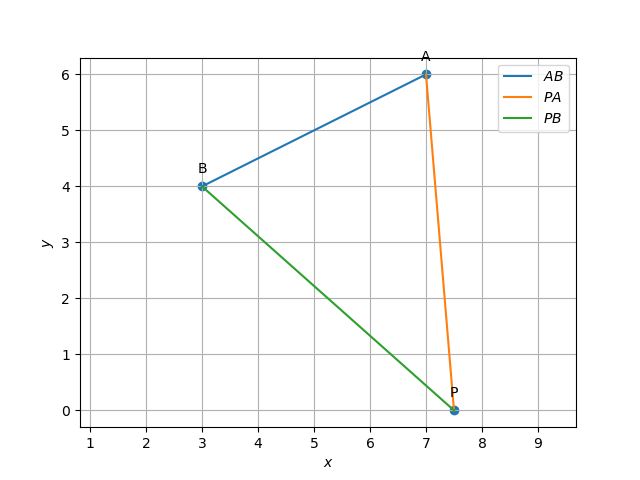
\includegraphics[scale=0.5]{Figure1.png}} \vspace{3mm}\centering

A$\begin{pmatrix}
  7 \\
  6 \\
 \end{pmatrix}$  $|A_0|$=$\sqrt{(7-x)^2+(6-0)^2}$\\ \vspace{2mm}
B$\begin{pmatrix}
  3 \\
  4 \\
 \end{pmatrix}$  $|B_0|$=$\sqrt{(3-x)^2+(4-0)^2}$\\ \vspace{1.5mm}
$|A_0|$=$|B_0|$\\                             \vspace{2mm}
$(7-x)^2+36=(3-x)^2+16$\\                     \vspace{1.5mm}
$(7-x)^2+20=(3-x)^2$\\                        \vspace{1.5mm}
$49+x^2-14x+20=9+x^2-6x$\\                    \vspace{1.5mm}
$60=8x$\\                                     \vspace{1.5mm}
$x=60/8$\\                                    \vspace{1.5mm}
$x=7.5$                                       \vspace{1mm}

\begin{mdframed}
https://github.com/hari1847/hari/blob/main/matrices
/hari.py
\end{mdframed}

\end{multicols}
\end{document}
